\documentclass{article}
\usepackage[T1]{fontenc}
\usepackage{helvet}
\renewcommand{\familydefault}{\sfdefault}
\usepackage{graphicx}
\usepackage{amsmath,amsthm,amssymb,latexsym}
\usepackage{enumerate}
\usepackage{hyperref}
\usepackage{url}

\newcommand{\no}{\noindent}
\newcommand{\bn}{\bigskip\noindent}
\newcommand{\sn}{\smallskip\noindent}
\newcommand{\mn}{\medskip\noindent}

\begin{document}
\begin{center}
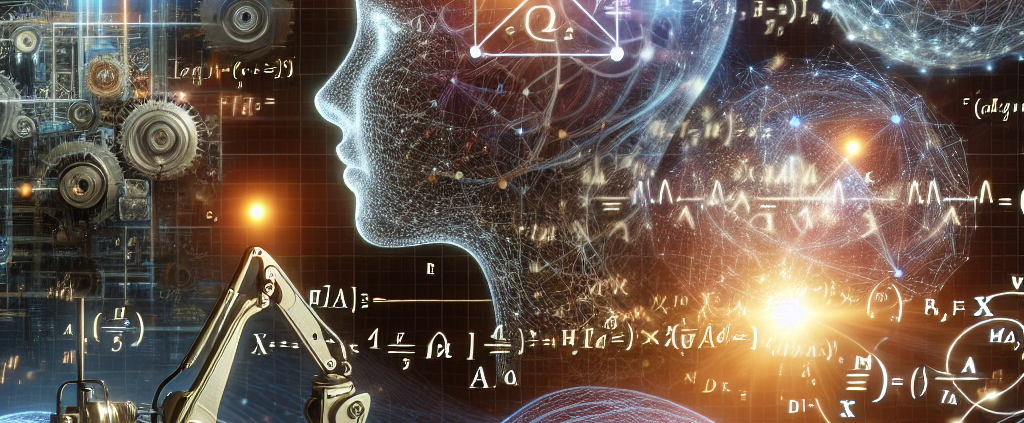
\includegraphics[scale=0.44]{fig/intelligence-knowledge-creation.png}
\end{center}

\mn
{\huge\bf Intelligence Activity and }

\bn
{\huge\bf Decision Probability Shifts }

\bn
{\huge\bf in Knowledge Creation}


\section*{Abstract}
Knowledge creation is not a static process; it emerges from the dynamic interplay between accumulated knowledge and decision probability. The Whole-in-One Framework (WIOF) introduces intelligence as a {\bf dynamic parameter}, demonstrating that intelligence does not just process knowledge but actively generates new knowledge by increasing decision probability. This process of knowledge creation is measured by the increase in decision probability, where the probability decision shift serves as the abstraction of intelligence. The activity of intelligence directly increases decision probability, enabling knowledge transformation and abstraction. The probability decision shift is the measure of the activity of intelligence. This article provides a simple and clear explanation of how decision probability shifts as intelligence operates, leading to higher levels of abstraction and understanding.

\section{Introduction}
In both human cognition and artificial intelligence (AI), decision-making is a probabilistic process influenced by accumulated knowledge. The Whole-in-One Framework proposes that intelligence creates new knowledge from accumulated knowledge, and this process is measured by the increase in decision probability. The activity of intelligence is what causes decision probability to shift, reinforcing the connection between intelligence and knowledge evolution. The probability decision shift is not only a transformation process but also an abstract measure of the active function of intelligence. This insight explains how intelligence evolves and how abstraction is formed through iterative decision-making.

\section{The Relationship Between Knowledge and\\ Decision Probability}
Decision probability is the likelihood of selecting the correct or optimal decision based on available knowledge. The Whole-in-One Framework defines this transformation mathematically as:

$$
D_i = \sigma(z) = \frac{1}{1+e^{-z}}
$$

\no
where:
\begin{itemize}
\item  $D_i \to$  Probability of making a correct decision.
\item $z\to$  Accumulated knowledge influencing decision-making.
\item  $\sigma(z)\to$ The sigmoid function, acting as the interface between knowledge and decision probability.
\end{itemize}

\\mn
At low levels of knowledge ($z$ is small), decision probability is also low. However, as intelligence processes and integrates knowledge, decision probability increases, leading to a higher certainty in selecting optimal outcomes. This increase in decision probability is directly caused by the activity of intelligence and serves as an abstraction of its function.

\section{Knowledge Creation as a Function of Decision Probability Shifts}
The fundamental equation describing how decision probability evolves with knowledge is:

$$
\frac{dD_i}{dz} = D_i(1 - D_i)
$$

\no
This equation describes a self-reinforcing loop:
\begin{itemize}
\item   When decision probability is low, new knowledge accumulation has little effect.
\item As decision probability increases through the activity of intelligence, new knowledge is integrated more efficiently.
\item  When a decision reaches high probability, it leads to the formation of abstract knowledge, allowing intelligence to make new connections beyond the initial problem space.
\end{itemize}


\subsection*{Example: How Intelligence Transforms Accumulated\\ Knowledge into New Knowledge}
Consider a researcher attempting to solve a differential equation that has never been solved before. This scenario illustrates how intelligence dynamically interacts with accumulated knowledge to generate new knowledge, measured by decision probability shifts.

\bn
{\bf 1. Initial State -- Low Decision Probability:}
\begin{itemize}
\item  The researcher starts with a {\bf probability of success at 45\% ($D = 0.45$)}, based on their accumulated knowledge in differential equations, mathematical techniques, and prior research.
\item At this stage, their ability to solve the equation remains uncertain, and they rely on existing knowledge frameworks.
\end{itemize}

\bn
{\bf 2. Active Processing -- Intelligence in Action:}

\begin{itemize}
\item  The researcher engages in {\bf deep analysis}, reviewing relevant literature, experimenting with different mathematical approaches, and leveraging problem-solving techniques.
\item This process {\bf integrates new insights}, refining their approach and testing various transformations to approach a solution.
\item  Each refinement {\bf increases their decision probability} as their accumulated knowledge is expanded and structured more effectively.
\end{itemize}

\bn
{\bf 3. Knowledge Expansion -- A Shift in Decision Probability:}
\begin{itemize}
\item  As the researcher {\bf formulates a breakthrough approach}, their decision probability shifts from {\bf 45\% to 55\% ($D = 0.55$)}.
\item This increase is not random; it is the direct result of intelligence processing accumulated knowledge and extracting new structural insights.
\item  The equation is solved, resulting in the {\bf creation of new knowledge that was previously inaccessible.}
\end{itemize}

\bn
{\bf 4. Recursive Impact  -- Intelligence as a Self-Reinforcing System:}
\begin{itemize}
\item  The newly acquired knowledge is now {\bf integrated into mathematical literature}, making it available for other researchers to build upon.
\item Future differential equations of similar nature can now be approached with a higher {\bf initial decision probability} due to this expanded knowledge base.
\item  This recursive process demonstrates how intelligence continuously expands the domain of knowledge by shifting decision probabilities.
\end{itemize}

\no
Every increase in decision probability represents an expansion in knowledge, demonstrating that intelligence actively {\bf creates new knowledge rather than merely processing existing information}. The probability decision shift is the direct result of intelligence in action and serves as an abstraction of intelligence itself.

\section{Intelligence as a Self-Reinforcing Knowledge\\ System}
From the above, intelligence can be modeled as a recursive learning system, where each decision probability shift feeds back into knowledge accumulation. The process can be summarized as:

$$
\frac{dz}{dt} = f(D_i)
$$

\no
where:
\begin{itemize}
\item  $\displaystyle \frac{dz}{dt}$ → The rate of knowledge accumulation over time.
\item $f(D_i)$ → A function showing how decision probability impacts knowledge creation.
\end{itemize}

\no
This shows that knowledge growth is proportional to decision probability increases---confirming that intelligence is not just a processor of existing knowledge but an engine for generating new knowledge. The activity of intelligence directly causes decision probability shifts, reinforcing knowledge expansion and abstraction. The probability decision shift is not only a transformation process but also a metric that abstracts the operation of intelligence.

\section{Conclusion: The Nature of Abstraction in\\ Intelligence}

\begin{itemize}
\item  Intelligence creates new knowledge from accumulated knowledge, and this process is measured by the increase in decision probability.
\item The sigmoid function acts as the mathematical transformer between raw knowledge and structured decision probability.
\item  Intelligence creates abstraction by continuously improving its decision probability, leading to new layers of understanding.
\item The probability decision shift is an abstraction that measures the activity of intelligence.
\item Intelligence functions as a dynamic parameter in knowledge evolution, with decision probability shifts being not only a measure of knowledge creation but also a measure of the activity of intelligence.
\end{itemize}

\no
This simple but profound insight applies to human learning, AI development, and even scientific discovery, showing that intelligence follows a structured path toward higher-order thinking. 

\bn
{\bf Future Work}: Expanding this framework to model AI learning systems, neuroscience, and decision-making in complex environments.

\bn
{\bf Final Thought}: Intelligence is not just about processing knowledge---it is about transforming probability into new knowledge, pushing the boundaries of abstraction forward.

\end{document}

\begin{itemize}
\item  
\item 
\item  
\item 
\end{itemize}
